\documentclass{article}
\usepackage[utf8]{inputenc}
\usepackage{graphicx}
\usepackage[francais]{babel}

\title{Compte Rendu - Projet Modélisation et Programmation C++}
\author{BAYET Théophile, MOUNE Paul}
\date{Mai 2017}

\begin{document}

\maketitle

\vspace{1.5cm}

\tableofcontents

\vspace{1.5cm}

\section{Introduction}

Ce document est le compte-rendu du projet de modélisation et programmation C++. Il regroupe les réponses aux questions des
différents TP ainsi que nos commentaires sur notre implémentation et diverses remarques. \\
L'objectif de ce projet est de modéliser et visualiser un océan.

\vspace{1cm}

\section{TP1}

L'objectif de ce TP est d'implémenter une classe Dvector qui sera ensuite utiliser dans notre modèle pour stocker les différentes hauteurs des points. \\

Nous avons donc créer plusieurs constructeurs ainsi que le destructeur. On retrouve le constructeur par défaut mais aussi un constructeur par recopie et un constructeur par lecture de fichier.

Nous avons aussi implémenter une méthode $display$ qui permet d'afficher sur la sortie standard l'objet de la classe Dvector.

\vspace{0.5cm}

\subsection{Questions :}

Considérons le code : \\ \\ $Dvector$ $x;$ \\ $x = Dvector(3, 1.);$ \\ \\

Ici, on construit d'abord un élément de la classe Dvector nommé x sans l'initialiser.
On utilise ensuite l'opérateur = qui a été redéfini pour la classe Dvector et qui va assigner à x une valeur.

En revanche, si l'on écrit directement : \\ \\ $Dvector x = Dvector(3, 1.);$ \\ \\

On construit directement le Dvector x avec une valeur en utilisant le constructeur adéquat que l'on a défini.


\vspace{1cm}

\section{TP2}

Le but de ce TP est d'enrichir notre classe Dvector créee lors du premier TP en implémentant différentes méthodes.

D'une part, il s'agit d'implémenter les opérateurs classiques pour qu'ils fonctionnent sur notre classe, comme par exemple l'addition avec un autre Dvector ou encore la multiplication par un scalaire.

Nous créons aussi un opérateur d'accession à un élément du Dvector. De plus, nous surchargeons les opérateurs d'affectation et de test d'égalité.

\vspace{0.5cm}

\subsection{Questions :}

\vspace{1cm}

\section{TP3}

Dans ce TP, nous allons déclarer plusieurs classes qui vont être utilisées pour modéliser l'océan.

Dans un premier temps, il nous faut une classe $Height$ qui va utiliser la classe Dvector que nous avons implémentée avant. Cette classe contiendra l'ensemble des valeurs des hauteurs claculées dans la "boîte" qui servira d'océan.

Ainsi, la classe Height est composée de 2 entiers, les dimensions de la boîte, et d'un Dvector de taille $DimX * DimY$.

Nous créons les différents constructeurs qui vont nous être utiles ainsi que le destructeur.

Les différentes méthodes implémentées pour cette classe sont les accesseurs aux dimensions et qu'un opérateur () permettant d'accéder à la valeur de la hauteur stockée en $(i,j)$.

De plus, nous avons besoin d'une méthode $set$ qui modifie la valeur de la hauteur en un endroit particulier.

Dans un second temps,  nous allons définir une classe mère, $WaveModel$, qui va nous servir pour implémenter l'effet des vagues dans l'océan. Plus tard, plusieurs classes hériterons de celle-ci.

Il ne faut pas que les différents paramètres de cette classe soient modifiables, ils sont donc privées et nous ne définissons pas de fonctions pour $set$.

En revanche, nous devons définir des accesseurs ainsi que plusieurs types de constructeurs.

De plus, nous implémentons un opérateur () qui permet de considérer cette classe comme un foncteur.

Enfin, nous implémentons une première modélisation de vague avec la classe $GernsterWaveModel$ qui dérive donc de la classe $WaveModel$.

\vspace{0.5cm}

\subsection{Question 2:}

Nous avons donc, dans notre implémentation de la modélisation de l'océan, créer plusieurs classes. Comme il existe plusieurs façons de représenter les vagues, la classe $WaveModel$ va être dérivée pour créer plusieurs modèles.

D'une part, on aura la classe $GernsterWaveModel$, qui héritera donc de la classe $WaveModel$. D'autre part, on aura aussi la classe $PhilipsWaveModel$, qui sera décrite dans la prochaine section, qui héritera de la même manière de la classe $WaveModel$.

De plus, la classe $Height$ qui va être utilisée dans nos modèles de vagues va contenir un tableau à 2 dimensions qui sera implémenté grâce à la classe $Dvector$ que nous avons créée au début.

\vspace{0.5cm}

\subsection{Question 3:}

Pour gérer l'apparence des vagues modélisées dans notre océan, plusieurs paramètres vont influencer la violence de la houle.

Ainsi, dans la classe $WaveModel$, nous pourrons contrôler la houle grâce aux paramètres d'intensité et de hauteur maximum de vague.

\vspace{1cm}

\section{TP4}

L'objectif de ce TP est de trouver et implémenter un nouveau modèle de visualisation de la houle dans l'océan.

Pour cela, nous allons utiliser une représentation spectrale du champ de hauteur. Nous créons donc une classe $PhilipsWaveModel$ qui dérive directement de la classe $WaveModel$ créer auparavant.

Pour cette représentation, il faut implémenter la transformée de Fourier ainsi que son inverse et l'appliquer sur notre champs de hauteurs.

On implémente donc la Fast Fourier Transform, FFT, avec l'algorithme de Cooley-Tukey. Pour pouvoir l'appliquer sur notre champ de hauteurs, il faut modifier la classe $Dvector$ que nous avons implémenté pour qu'elle gère une partie imaginaire.


Maintenant que la classe est créée et l'implémentation de la FFT faite, il nous faut maitenant créer la classe Océan qui va nous servir pour regrouper tout le travail fait et permettre la visualisation de notre modèle.

On lui donne en paramètres les différentes dimensions nécessaires à la modélisation et à la visualisation, ainsi que le temps, le modèle de houle utilisé avec un paramètre de la classe $WaveModel$ et un Dvector qui contient les hauteurs de la houle.

\vspace{1cm}

\section{Tests}

Toutes les classes et leurs méthodes qui ont été présentées ici ont été testées par plusieurs tests pertinents afin de veiller à ce que notre implémentation soit correcte.

Ces tests vont en effet tester pour toutes les classes implémentées les constructeurs, les operateurs et les méthodes propres à chaque classe.

Nous avons dans un premier temps un fichier de tests pour la classe $Dvector$.

\vspace{0.5cm}

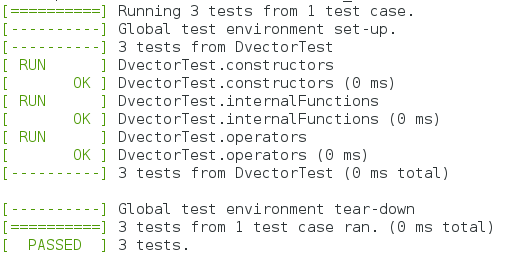
\includegraphics[scale=0.7]{./res/Test_Dvector.png}

\vspace{0.5cm}

De même, nous avons un fichier de tests pour les classes Height, Ocean et les différentes implémentations des vagues.

\vspace{0.5cm}

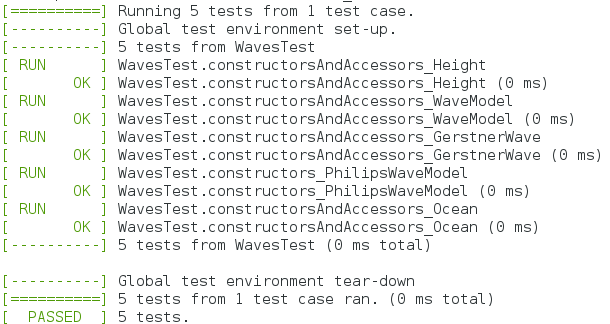
\includegraphics[scale=0.7]{./res/Test_Waves.png}

\vspace{1cm}


\section{Visualisation et résultats}

\vspace{1cm}

\section{Commentaires}


\end{document}
